\subsubsection{Gitterstruktur und Elektronendichteverteilung}

In diesem Abschnitt soll die  Elektronendichteverteilung und die Gitterstruktur des Graphit untersucht werden. Daf�r wurde ein kleiner Bereich herangezoomt, damit die atomare Struktur sichtbar wird. Es wurde ein Bereich von 3 x 3 nm verwendet, der m�glichst glatt erscheint. Die Verkippung der Probe wurde korrigiert, die Aufnahme ist in Abbildung \ref{fig:graphit_atomstruktur} zu sehen.

\begin{figure}[H]
\begin{subfigure}[t]{0.49\textwidth}
\includegraphics[scale = 0.7]{graphit_3nm_nanostruktur_oberflaeche.png}
\caption{Oberfl�che der Graphitprobe bei atomarer Aufl�sung. Es l�sst sich die hexagonale atomstruktur erkennen.}
\label{subfig:graphit_atomstruktur_1}
\end{subfigure}
\hspace{0.02\textwidth}
\begin{subfigure}[t]{0.49\textwidth}
\includegraphics[scale = 0.7]{graphit_3nm_nanostruktur_topographie.png}
\caption{Beispielhafter topologischer Verlauf, entlang der x-Achse}
\label{subfig:graphit_atomstruktur_2}
\end{subfigure}
\caption{Aufnahme der Oberfl�chen von Graphit in einem Bereich von 3 x 3 nm. Die H�hendifferenz liegt im Bereich von \SI{1,5}{\angstrom} }
\label{fig:graphit_atomstruktur}
\end{figure}

Um die Gitterstruktur noch besser sehen zu k�nnen, wird die Oberfl�che im Constant Hight Mode gescannt. Daf�r werden der P$_{gain}$ und der I$_{gain}$ auf die Werte in Tabelle \ref{tab:para_tip_graph} gesetzt.

\begin{table}[H]
\centering
\caption{Parameter zur Topographiemessung (CC-Mode)}
\begin{tabular}{c|c}
Variable & Wert\\
\hline Set point & \SI{1}{nA}\\
P-gain & 0\\
I-gain & 4\\
Tip-voltage & \SI{50}{mV}\\
\end{tabular}
\label{tab:para_tip_graph}
\end{table}

F�r den Scan wurde eine Fl�che von 1,1 x 1,1 nm gew�hlt. Die Aufnahme, mit eingezeichneter hexagonaler Struktur ist in Abbildung \ref{fig:graphit_1_1_nm_struktur} zu sehen. Die Aufnahme wurde geschert, damit die Gitterstruktur besser zu erkennen ist.

\begin{figure}[H]
\centering
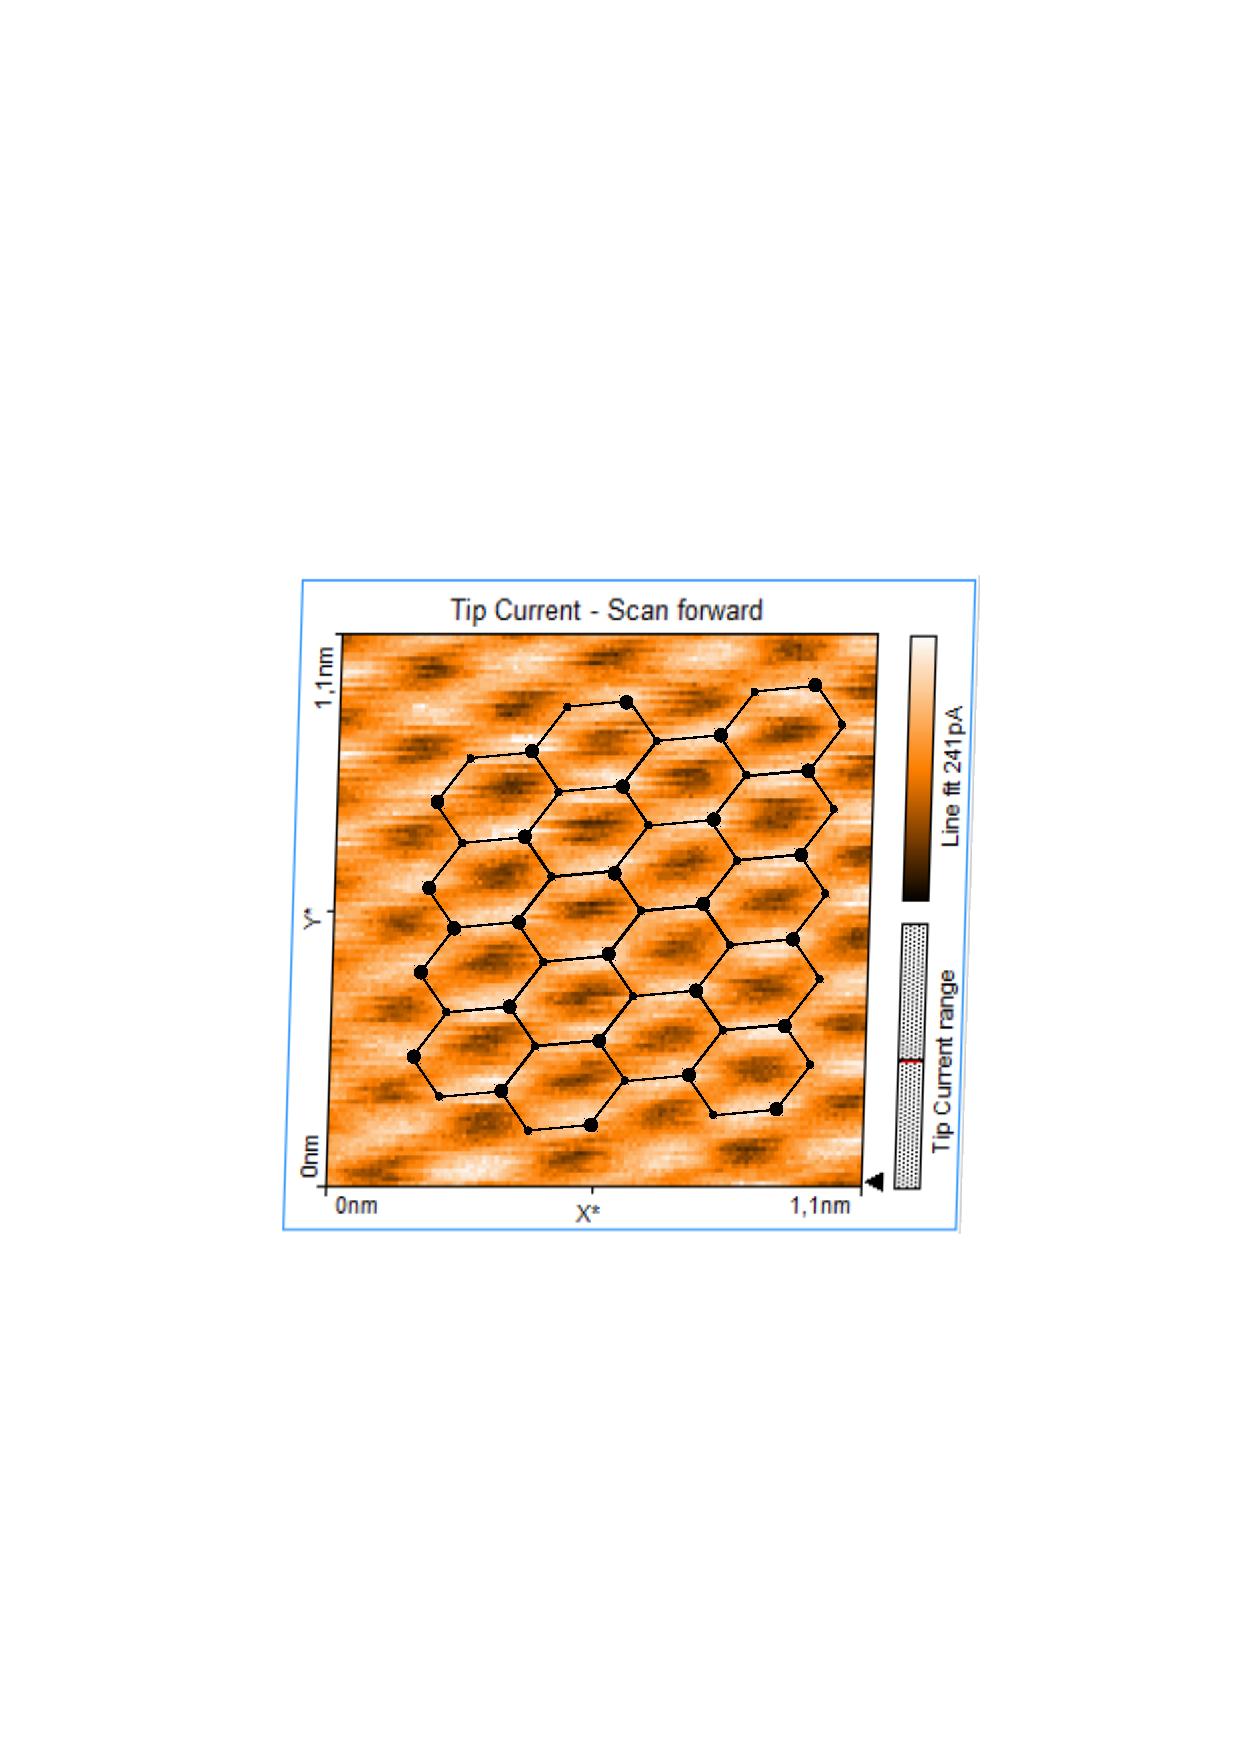
\includegraphics[trim = 10mm 128mm 10mm 135mm, clip=true, scale = 0.75]{graphit_1,1nm_CHM_struktur.jpg}
\caption{Aufnahme der Oberfl�che im Bereich von 1,1nm x 1,1nm. Zur Veranschaulichung wurde die Gitterstruktur eingezeichnet.}
\label{fig:graphit_1_1_nm_struktur}
\end{figure}

Abbildung \ref{fig:graphit_1_1_nm_struktur} ist so zu interpretieren, dass an den hellen Stellen die Gitteratome ohne Verbindungen zur darunterliegenden Schicht liegen, daher liegen die Elektronen direkt am Atom an und es wird ein h�herer Tunnelstrom gemessen. An den orangen Stellen befinden sich die Atome mit einer Verbindung zur darunterliegenden Schicht, wodurch der Tunnelstrom geringer wird. Die schwarzen Bereiche entsprechen der Mitte der Hexagons, bei welchen das n�chste Atom erst in der darunterliegenden Schicht liegt, sodass der Tunnelstrom sehr gering ist. In Abbildung \ref{fig:graphit_1_1_nm_struktur_3d} ist eine dreidimensionale Ansicht der Oberfl�che zu sehen.

\begin{figure}[H]
\centering
\includegraphics[scale = 0.75]{1,1x1,1_3d_plot}
\caption{3D Aufnahme der Oberfl�che im Bereich von 1 x 1 nm.}
\label{fig:graphit_1_1_nm_struktur_3d}
\end{figure}
